\section{研究领域和代码编写示例}
% ------------------------------------------------------------------------------------ %
\subsection{图像识别(Computer Vision)}
% ------------------------------------------------ %
% ------------------------------------------------ %




% ------------------------------------------------------------------------------------ %
\subsection{自然语言处理(Natural Language Processing)}
% ------------------------------------------------ %
% ------------------------------------------------ %

\subsubsection{情感分析}
帮助用户快速获取、整理和分析相关的评价体系，对带有感情色彩的主观性文本进行、处理、归纳和推理。
\begin{figure}[!h]
	\label{fig:Sentiment_Analysis_Process}
	\centering
	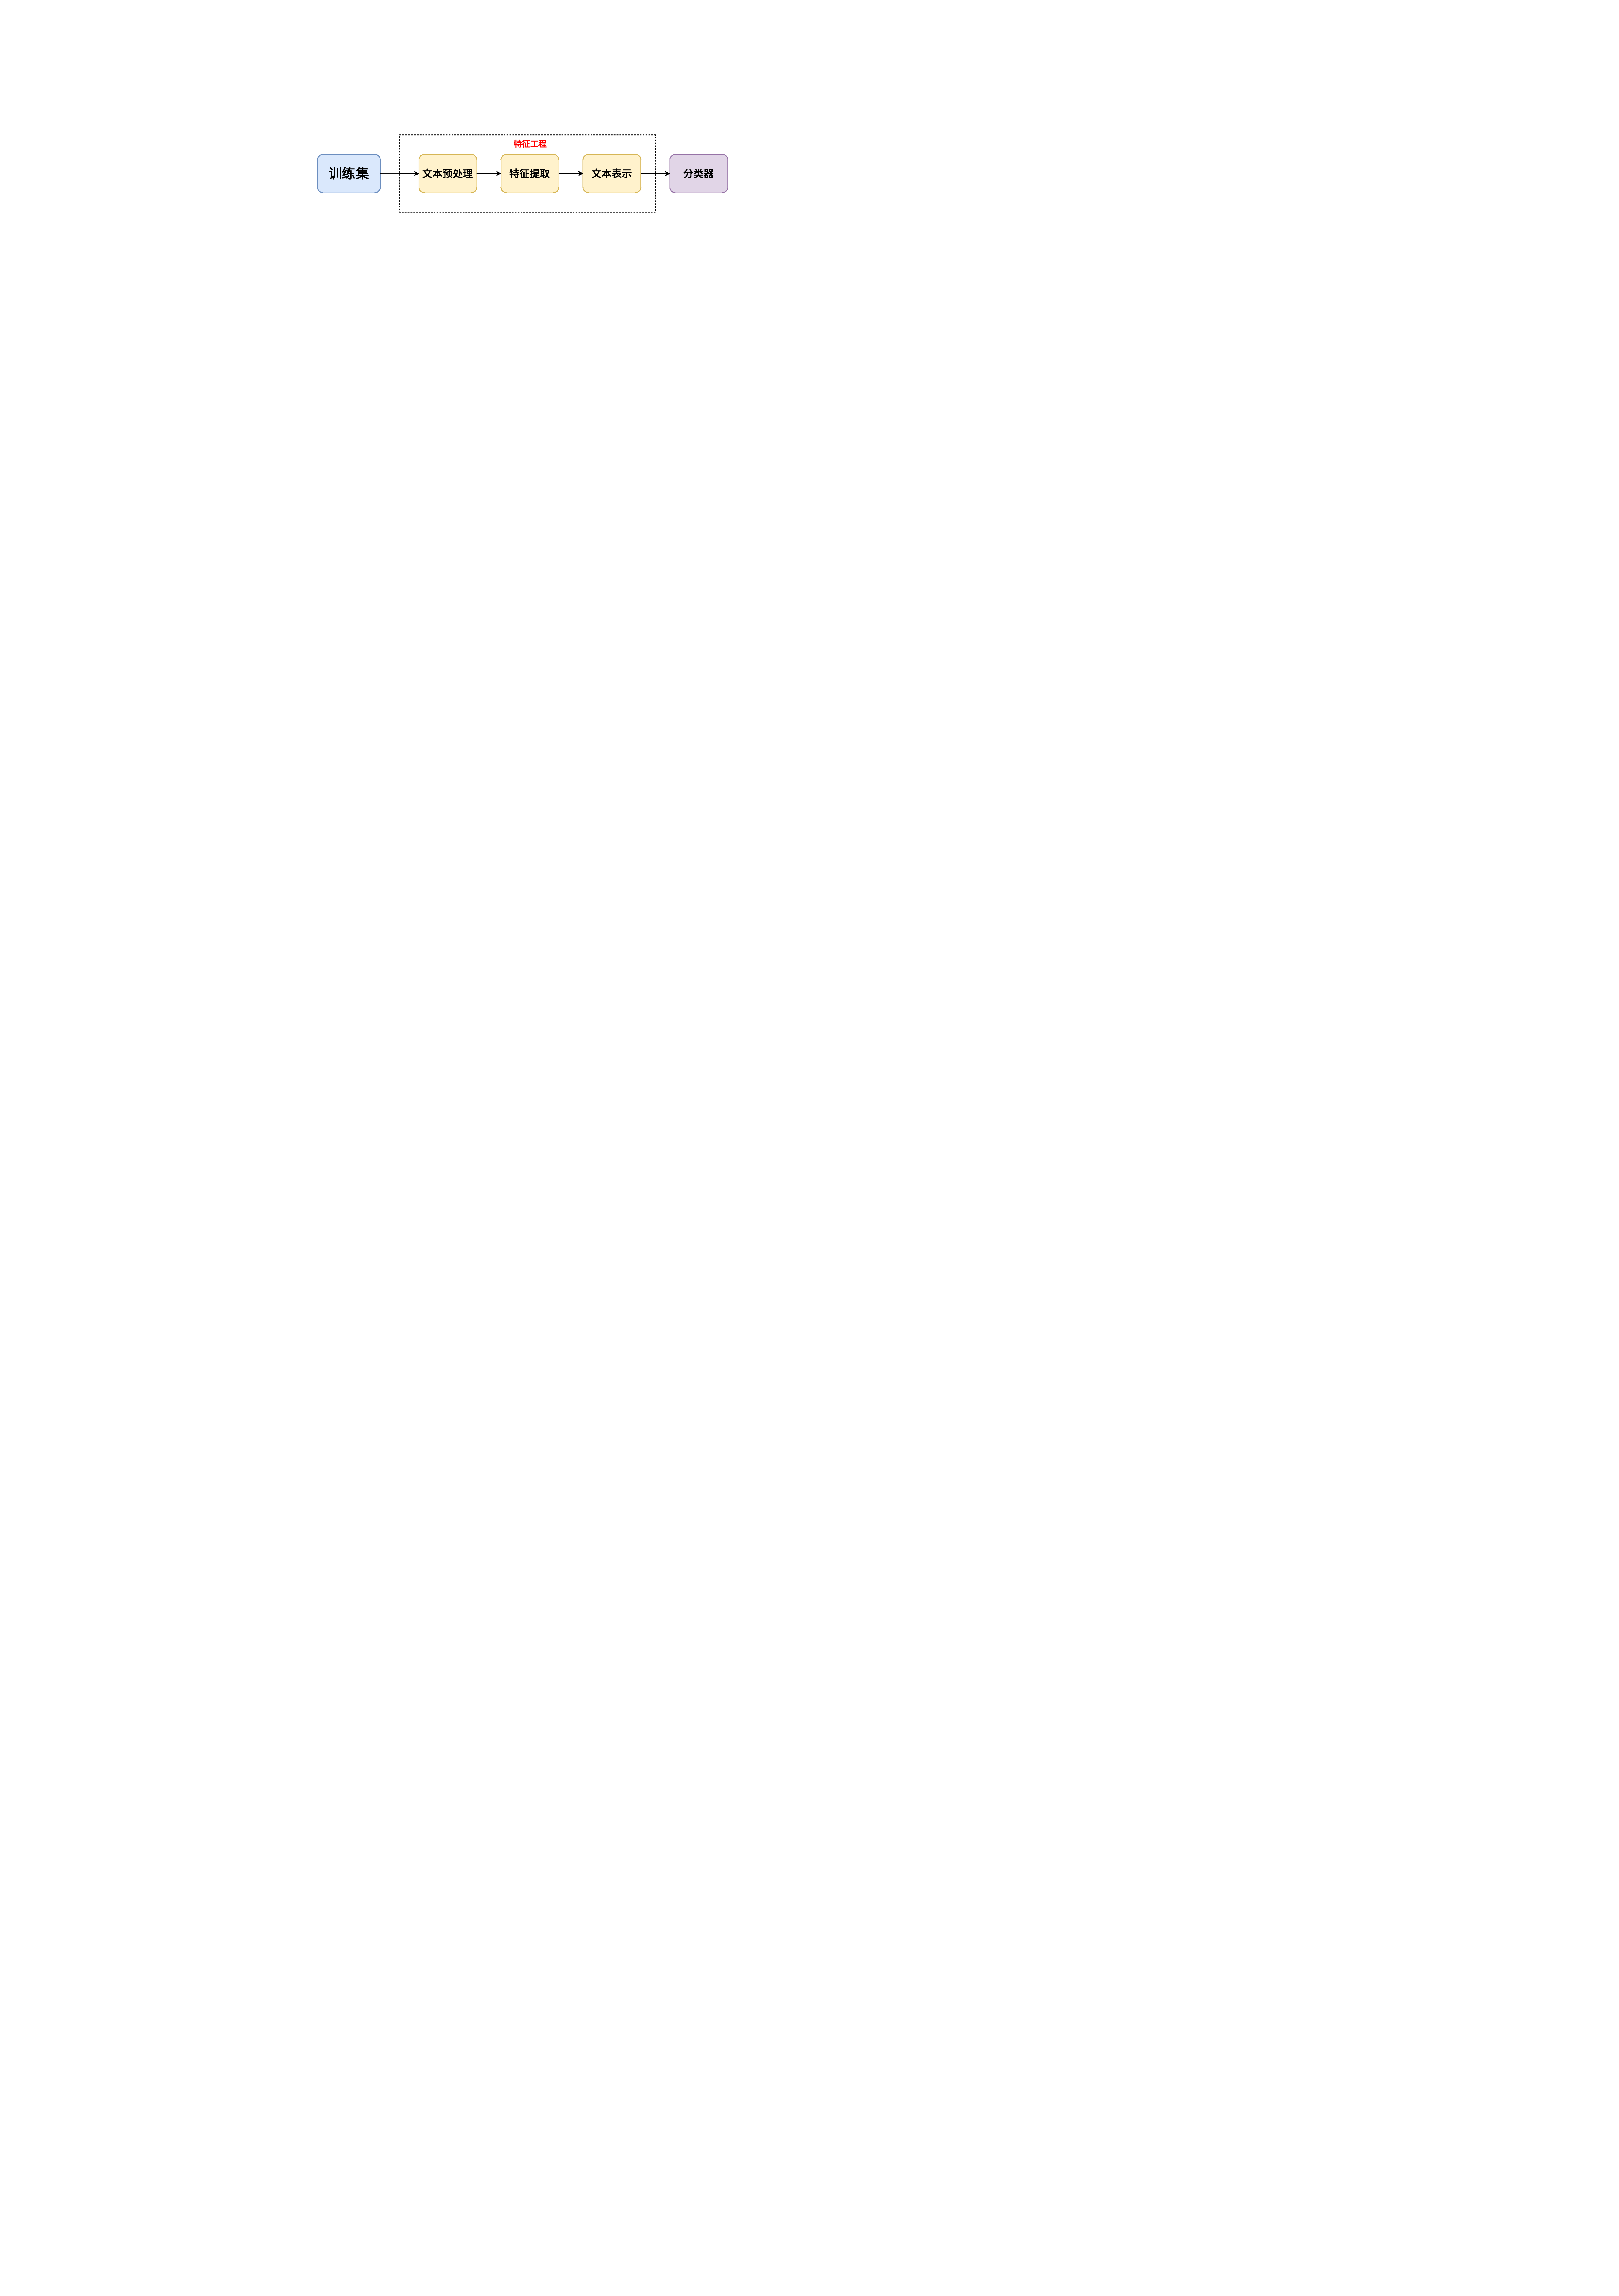
\includegraphics[scale=0.7]{Images/Chapter3_images/Sentiment_Analysis_Process.pdf}
	\caption{情感分析基本流程}
\end{figure}





% ------------------------------------------------------------------------------------ %
\subsection{生成式学习(Generative Learning)}
% ------------------------------------------------ %
% ------------------------------------------------ %


% ------------------------------------------------------------------------------------ %
\subsection{多模态(Multimodal)}
% ------------------------------------------------ %
% ------------------------------------------------ %







% ------------------------------------------------------------------------------------ %
\subsection{脉冲神经网络相关(SNN)}
% ------------------------------------------------ %
% ------------------------------------------------ %







